\subsubsection{\acl{pcl}}\label{subsec:PCL}

\citet{PCL_2021} use clustering in the feature space to optimize the sample's representation.
They assign multiple prototypes of different granularity to each sample.
The prototypes are found by clustering and 
they are considered positive samples.
The sample's embedding is enforced to be similar to those of its prototypes by a contrastive loss.
The so-called prototypical contrastive loss ProtoNCE is optimized using an \ac{em} algorithm 
as displayed in \autoref{fig:PCL_training}.
The prototypes are latent variables.

\begin{figure}[!htb] % h = here, t = top, b = bottom, p = page of floats
    \centering
    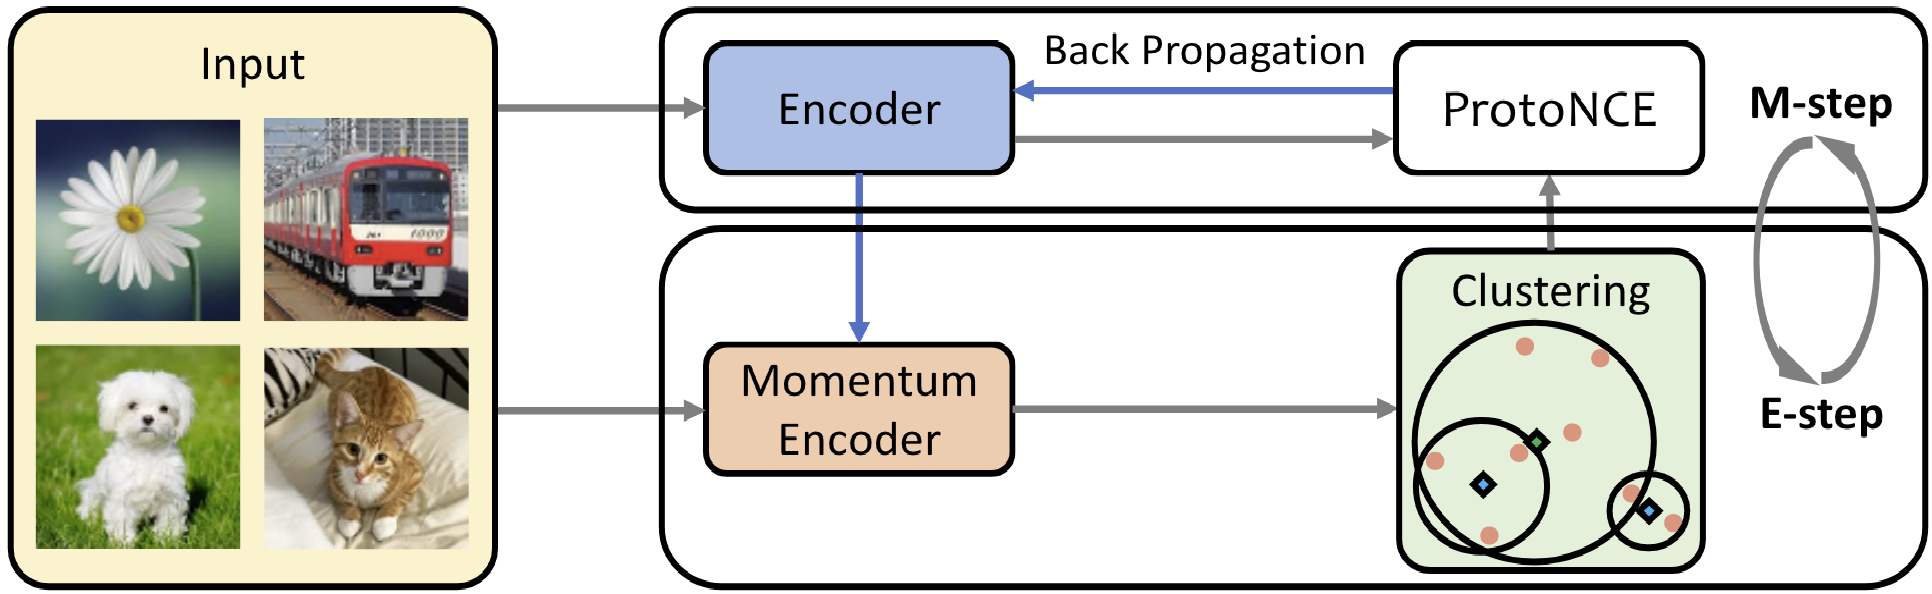
\includegraphics[width=360pt]{images/PCL_training.png}
    \caption{Illustration from \citet{PCL_2021}.
    The training of the \ac{pcl} algorithm is shown.
    $M$ $k_m$-means clusterings based on the feature space defined by the momentum encoder 
    are performed in the E-step.
    The prototypes $c^m_{\tilde{k}}$, $\tilde{k} \in [1, k_m]$, illustrated as green/ blue rectangles, 
    are the cluster centroids.
    The M-step updates the network parameters $\theta$ by optimizing the ProtoNCE loss.
    }
    \label{fig:PCL_training}
\end{figure}

% E-step: define k clusters & momentum encoder
$k$-means clustering is used to find the prototypes in the E-step.
The clustering is performed on the samples' embeddings obtained from the momentum encoder, 
whose parameters are a moving average of the main encoder's parameters and thus, smoother \citet{PCL_2021}.
The prototypes are the cluster centroids.

% M-step
The M-step updates the network parameters $\theta$ by optimizing the ProtoNCE loss.
The minimization of the ProtoNCE loss is equivalent to maximizing the estimated log-likelihood.
The optimal parameters are those that map a sample close to its prototypes.
The result is obtained under the assumptions of a uniform prior over the cluster centroids, i.e. prototypes,
and an isotropic Gaussian distribution of the sample's embeddings around the prototypes.

% ProtoNCE loss
The ProtoNCE loss from \eqref{eq:ProtoNCE} extends the InfoNCE from \eqref{eq:InfoNCE} 
by not only enforcing similarity between the sample and 
one positive sample while retaining dissimilarity to $r$ negative samples, 
but also considering its prototypes $c^m_s$. 
To improve the stability of the results, $M$ clusterings with different numbers of clusters $k_m$ are 
executed.
Different numbers of clusters lead to different granularity of the prototypes 
and thus, a hierarchical structure is encoded into the loss function.

\begin{equation}
    \mathcal{L}_{InfoNCE}= - \sum_{i=1}^{N}\log\frac{\exp \frac{z_i\cdot z_i'}{\tau}}{\sum_{j=0}^{r}\exp \frac{z_i\cdot z_j'}{\tau}}
    \label{eq:InfoNCE}
\end{equation}

\begin{equation}
    \mathcal{L}_{ProtoNCE}=\mathcal{L}_{InfoNCE} - \sum_{i=1}^{N} \frac{1}{M} \sum_{m=1}^{M} \log\frac{\exp \frac{z_i\cdot c_s^m}{\phi^m_s}}{\sum_{j=0}^{k_m}\exp \frac{z_i\cdot c_j^m}{\phi^m_j}}
    \label{eq:ProtoNCE}
\end{equation}


